\documentclass{article}

\usepackage[preprint]{neurips_2026}

\usepackage[utf8]{inputenc}
\usepackage[T1]{fontenc}
\usepackage{hyperref}
\usepackage{url}
\usepackage{booktabs}
\usepackage{amsfonts}
\usepackage{amsmath}
\usepackage{nicefrac}
\usepackage{microtype}
\usepackage{xcolor}
\usepackage{graphicx}

% Fill these in before submitting to OpenReview.
\newcommand{\CODABENCHID}{1039673}
\newcommand{\REPOURL}{\url{https://github.com/VihanAggarwal/paiec-2026}}
\newcommand{\CODABENCHSCORE}{\textbf{[CODABENCH SCORE]}}

\title{Pooling Revealed Labels with a Per-Benchmark Gaussian-Process Logistic Model: an Entry to the Predictive AI Evaluation Competition}

\author{%
  Vihan Aggarwal\\
  Millburn High School\\
}

\begin{document}

\maketitle

\begin{abstract}
We predict the probability that an AI system answers an item of a never-seen benchmark correctly,
given system and item attributes and a small budget of revealed labels. Our predictor has three
parts. (i) For each benchmark in the revealed evidence, a Gaussian-process logistic model is fitted
by a Laplace approximation to all revealed labels on that benchmark (any system). It combines
benchmark, system-benchmark pair and item-similarity terms, and integrates over posterior
uncertainty so that zero-label predictions are calibrated. (ii) An LLM difficulty judge (Claude
Sonnet 5.5) rates each item, and the rating enters the model's prior mean and kernel. (iii) An
in-context LLM judge (Claude Sonnet 5.5) sees the revealed outcomes on the benchmark and predicts
the new item, and is blended with the model; at budget 0 it is queried zero-shot. On a local evaluator that reproduces the official protocol with
leave-benchmarks-out cross-validation (541 pairs, 151 held-out benchmarks), parts (i) and (ii) reach
Brier ALC 0.1998, against 0.2500 for a constant 0.5 and 0.2426 for the official empirical-mean
baseline. On 97 held-out pairs, part (iii) lowers ALC by an estimated further 0.010 (0.014 when
Claude Opus 5.5 serves as the in-context judge at low budgets, a variant we validated but could not
run on the platform before the deadline). We also report
negative results. System ability inferred from the model name does not transfer across benchmarks
($r=-0.07$). Text features and sentence embeddings do not predict item difficulty on new benchmarks
($r\approx0.02$ to $0.04$ within benchmarks), whereas LLM ratings do ($0.20$ to $0.24$). And one
formative leaderboard score has a standard deviation of about 0.047, so single draws say little about
a method.
\end{abstract}

\section{Introduction}

Decision makers often need to know how well an AI system will do on a new task before running it
exhaustively. The Predictive AI Evaluation Competition (PAIEC) \citep{paiec_site} turns this into a
prediction problem. A \emph{subject} is an AI system configuration (model, harness, harness version,
reasoning effort). An \emph{item} is a benchmark question. For each target subject-item pair, the
submitted program returns $P(\text{correct})$ from the subject and item attributes and from the
\emph{revealed labels} available at the current budget. Test benchmarks are disjoint from training
benchmarks (benchmark-level cold start). Labels are revealed at budgets $n \in \{0,1,3,7,15,31\}$ per
subject-benchmark pair, and the score is the Brier area under the learning curve,
\begin{equation}
\mathrm{ALC} = 0.1\,B_0 + 0.2\,(B_1 + B_3 + B_7 + B_{15}) + 0.1\,B_{31},
\end{equation}
computed per pair and averaged with equal weight over pairs \citep{brier1950}. A constant 0.5 scores 0.25.

Our contributions are practical:
(i) a local evaluator that reproduces the official streaming protocol on the public training data
with leave-benchmarks-out cross-validation, checked by an independent review;
(ii) a per-benchmark Gaussian-process (GP) logistic classifier with Laplace inference
\citep{williams1998,rasmussen2006}, which subsumes the usual pooling estimators as special cases and
gives calibrated uncertainty at every budget;
(iii) two uses of an LLM that transfer to unseen benchmarks: an item-only difficulty judge inside the
GP, and an in-context judge that reads the revealed outcomes on the benchmark. Both are validated
against held-out data, and both fall back to the plain model when the API is unavailable;
(iv) ablations and negative results (subject priors, amortized item difficulty from text and
embeddings, empirical Bayes), an analysis of how noisy one formative leaderboard score is, and a
packaging bug that we found and fixed.

\section{Data}

\paragraph{Source.} We use only the competition's public training release, the gated Hugging Face
dataset \texttt{aims-foundations/measurement-db} \citep{measurementdb}, which is part of the
benchmark inventory. We downloaded revision \texttt{54074453} (tables only: benchmarks, subjects,
items, responses; no traces or media). No other data, pretrained model or external API is used.

\paragraph{Selection.} Of 281 benchmark folders, 278 are public. We keep the 167 public, item-level
benchmarks whose recorded responses are all 0 or 1. Of these, 156 are typed \texttt{binary}; 11 have
another type, but every recorded response in them is 0 or 1. The kept data contain 68.8M responses
(about half are repeated trials), 14,483 subject IDs, 707 distinct
\texttt{normalized\_name} values, 3.67M items and 14,735 subject-benchmark pairs. 13,200 of those
pairs have at least 80 distinct items, the platform's threshold for test-time acquisition. The mean pair
accuracy is 0.549 (standard deviation 0.268).

\paragraph{Mapping to the predictor input.} The subject dictionary is the subjects table's eight
fields (missing values become \texttt{""}). The item's \texttt{item\_content} is the items table's
\texttt{content} (sometimes a JSON list of multimedia elements), \texttt{item\_features} is a
\texttt{key=value;...} string, \texttt{interactors} comes from the response, and \texttt{benchmark\_id}
is anonymous on the platform. Subject IDs are almost always specific to one benchmark (only 236
appear in more than one), and harness strings are mostly benchmark-specific, so a subject can be
linked across benchmarks only through its model name.

\section{Method}

\paragraph{Model.} Let $b$ be a benchmark, $s$ a subject and $i$ an item. The latent logit of a
correct response is
\begin{equation}
f(s,i) = \mu_0 + \beta_b + \gamma_{s,b} + g(i),
\end{equation}
with independent zero-mean Gaussian-process priors on the benchmark offset $\beta_b$ (variance
$\tau_b^2$), the pair offset $\gamma_{s,b}$ (variance $\tau_p^2$) and the item term $g$, whose
covariance is a sum of two cosine kernels:
\begin{equation}
k\big((s,i),(s',i')\big) = \tau_b^2 + \tau_p^2\,\mathbf{1}[s=s'] + \tau_f^2\cos\!\big(\phi_F(i),\phi_F(i')\big) + \tau_t^2 \cos\!\big(\phi_T(i),\phi_T(i')\big),
\end{equation}
for two items of the same benchmark. v6 adds $\tau_m^2\cos(\bar e_i,\bar e_{i'})$, where $\bar e_i$
is the item's all-MiniLM-L6-v2 sentence embedding minus the mean embedding of the benchmark's
revealed items (the target is centred with the same mean). Here $\phi_F$ is an IDF-weighted binary vector of the
\texttt{item\_features} tokens (\texttt{key=value} parts and interactors), and $\phi_T$ is a TF-IDF
vector of lower-cased alphanumeric tokens of the first 4,000 characters of \texttt{item\_content}.
IDF weights come from the revealed items of that benchmark, and the norm of each vector
includes tokens unseen among them. Responses are $y \sim \mathrm{Bernoulli}(\sigma(f))$. An optional
exact-item term $\tau_e^2\mathbf{1}[i=i']$ and a subject prior mean $u(s)$ are evaluated as
ablations.

\paragraph{Inference.} Given the $m$ revealed labels $\mathbf{y}$ of benchmark $b$ (all subjects),
we find the posterior mode $\hat{\mathbf{f}}$ by Newton's method (Algorithm 3.1 of
\citet{rasmussen2006}) with prior mean $\mu_0$, and set $W=\mathrm{diag}(\hat\pi(1-\hat\pi))$ and
$B = I + W^{1/2} K W^{1/2}$. For a target with kernel vector $\mathbf{k}_*$ and prior variance $k_{**}$,
\begin{align}
\bar f_* &= \mu_0 + \mathbf{k}_*^\top(\mathbf{y}-\hat{\boldsymbol\pi}), &
v_* &= k_{**} - \mathbf{k}_*^\top W^{1/2}B^{-1}W^{1/2}\mathbf{k}_*, &
p_* &= \sigma\!\Big(\bar f_* \big/ \sqrt{1+\pi v_*/8}\Big),
\end{align}
the last step being the probit approximation to $\mathbb{E}[\sigma(f_*)]$ \citep{mackay1992}.
With no revealed label on the benchmark (always at budget 0), $p_* = \sigma(\mu_0/\sqrt{1+\pi k_{**}/8})$.
Labels of other subjects on the same benchmark inform $\beta_b$ and the item terms. The target
pair's own labels additionally inform $\gamma_{s,b}$.

\paragraph{Versions (nested ablations).}
\textbf{v0}: the official empirical-mean baseline \citep{paiec_baselines}.
\textbf{v1}: prior only, $\mu_0 + u(s)$, where $u$ is a shrunk mean residual of the subject's model name
(provider as fallback) over training benchmarks.
\textbf{v2}: adds $\beta_b$ (no pair term).
\textbf{v3}: adds $\gamma_{s,b}$.
\textbf{v4}: adds the item kernels and drops $u(s)$.
\textbf{v4b}: v4 plus an identical pure-Python solver used only if numpy is missing.
\textbf{v5}: v4b with the prior mean lowered from $\mu_0$ to $\mu_0-0.8$ (Section~\ref{sec:results}).
\textbf{v6}: v5 plus the semantic kernel ($\tau_m=1$, with $\tau_t$ lowered to 0.5).
\textbf{v7}: v6 plus the LLM difficulty judge described next, with Claude Haiku 5.5.
\textbf{v8}: v7 with Claude Sonnet 5.5 as the judge (slope refitted on its ratings).
\textbf{v9}: v8 plus the in-context judge below.
\textbf{v10}: v9 with the in-context judge also queried at budget 0, with an empty context (submitted).
\textbf{v11}: v10 with Claude Opus 5.5 as the in-context judge (weight 0.8) while the target has 1
to 7 revealed labels (validated locally; not run on Codabench before the deadline).

\paragraph{In-context judge (v9).} The item-only judge cannot know what an outcome of 1 means on a
new benchmark, how strong the target system is, or which kinds of item it fails. The revealed labels
answer all three. For each target at budget $n\ge1$, Sonnet 5.5 receives the target system's revealed
items with their outcomes (up to 31; item text truncated to 400 characters), other systems' revealed
items on the same benchmark (up to 24), and the new item (1,200 characters). It is told to anchor on
the target's observed rate and to infer the meaning of outcome 1 from the examples, and it returns
$\hat p_{\mathrm{LLM}}$. The prediction is $p=(1-w)\,p_{\mathrm{v8}}+w\,\hat p_{\mathrm{LLM}}$ with
$w=0.65$. At budget 0, or when the call fails, $p=p_{\mathrm{v8}}$. Calls have their own 30-minute
time budget per worker process, and the item judge's budget is lowered to 20 minutes, so six
budgets stay inside the 8-hour limit.

\paragraph{LLM difficulty judge (v7).} For each item, Claude Haiku 5.5 (\texttt{claude-haiku-5-5},
Anthropic Messages API, no extended thinking, structured JSON output) is asked for the probability,
0 to 100, that ``a typical current AI model'' answers the item correctly or succeeds, given the item
text (first 1,500 characters) and features. The rating $r_i$ becomes a logit
$z_i=\log\frac{r_i+2}{102-r_i}-c$, centred by the training mean $c$. It enters the model twice:
the prior mean gains $s\,\gamma\,z_i$, and the kernel gains $\tau_j^2 z_i z_{i'}$, which lets the
revealed labels of a benchmark adjust the judge's slope there. Here $\gamma=0.20$ is the slope of
an item's mean-response logit on $z$ across training benchmarks (refitted per fold), and $s=2$ and
$\tau_j=0.6$ were chosen on the local evaluator among $s\in\{1,2,3\}$, $\tau_j\in\{0,0.6\}$.
Ratings are cached per item. Revealed items of a benchmark are rated concurrently (8 threads), calls
time out after 10\,s with one retry, and a per-process time budget switches the judge off; any
failure or a missing key gives $z_i=0$, which is exactly v6. v8 calls Sonnet 5.5
(\texttt{claude-sonnet-5-5}) with the same prompt and settings; its fitted slope is $\gamma=0.27$.
The time budget is 40 minutes of API time per worker process, so six budgets stay well inside the
8-hour limit even if every rating is a cache miss.
We also evaluate a nonparametric empirical-Bayes alternative \citep{robbins1956}. A revealed label is
a response on a random item, so it is Bernoulli($q$) in the pair accuracy $q$. The prediction is
$\mathbb{E}[q\mid k,n,K,N]$ under a kernel-smoothed prior $g(q)$ fitted on training pairs, with
peers' successes $K$ of $N$ down-weighted by $w$.

\paragraph{Hyperparameters.} $\mu_0$ is the benchmark-weighted mean pair logit on the training
benchmarks ($-0.031$ for the full fit). The starting values $\tau_b = 1.51$, $\tau_p=0.97$ are the
between- and within-benchmark standard deviations of the pair logits. The final values
$\tau_b=2.2$, $\tau_p=1.0$, $\tau_f=\tau_t=1.0$, $\tau_e=0$ (v4) were chosen by grid search on the
local evaluator (33 configurations in total). v6 uses $\tau_t=0.5$, $\tau_m=1.0$ and prior shift
$-0.8$, each chosen among a handful of settings. Every configuration near the optimum lies within 0.001 ALC
of it (Section~\ref{sec:results}).

\paragraph{Implementation.} \texttt{predict} caches the posterior per (evidence fingerprint,
benchmark), so each benchmark is solved once per budget. A target then costs $O(m^2)$. Solves are
capped at 1,500 labels per benchmark by a deterministic subsample. The submitted \texttt{model.py}
needs only numpy, loads a 24\,KB JSON state, is deterministic and makes no network calls. In the
local smoke test it averages 0.03\,ms per call (0.22\,ms with the pure-Python fallback).
For v6 we re-implemented the MiniLM encoder (WordPiece tokenizer and 6-layer BERT forward pass) in
numpy, with float16 weights (42\,MB) bundled in the submission. It reproduces sentence-transformers
exactly on our checks (cosine 1.00000 on 48 items) and costs 39\,ms per item on one CPU thread.
Embeddings are cached per item, the semantic kernel is skipped for benchmarks with more than 400
revealed labels, and any encoder failure falls back to v5's predictions.

\section{Experimental setup}
\label{sec:setup}

\paragraph{Local evaluator.} Benchmarks are assigned to 7 folds with a fixed seed. For each fold,
the prior is refitted on the other folds' benchmarks only, and \texttt{model.py} is imported with
that fold's state. For each held-out benchmark with a pair of at least 80 items, we sample up to 8
subjects. Each takes 80 to 400 items from one benchmark-level random item order, all trials
included. Up to 4 pairs per benchmark are scored. Pairs are grouped 1 to 3 per benchmark and packed
into \emph{snapshots} of at most about 1,000 subject-item pairs, mirroring one formative evaluation.
The result is 159 snapshots of 3.4 pairs on average: 541 pairs from 151 benchmarks.
Within a pair, items are split 50/50 into acquisition and evaluation pools. The default split is
per pair (an item can be an acquisition item for one subject and an evaluation item for another).
The robustness check splits per benchmark. Acquisition follows a random order, one recorded
response is revealed per acquired item, and label sets are nested. At budget $n$,
\texttt{labeled} holds the first $n$ acquisitions of \emph{every} pair in the snapshot, in the
official \texttt{[[subject, item], label]} format. \texttt{predict} is called once per distinct
input. Brier scores use all evaluation responses (trials included), and ECE uses 10 equal-width bins
per pair. Constant 0.5 scores exactly 0.2500 (sanity check). Three independent reviewers, each with
an adversarial verification step, checked the evaluator for protocol deviations, leakage and metric
errors and confirmed no defect. The minor deviations they found (the parity of the split hash, 3 of
159 snapshots exceeding the cap by at most 95 items, 9 non-\texttt{binary}-typed benchmarks) each move
ALC by less than 0.0002 and change no ranking.

\section{Results}
\label{sec:results}

\begin{table}[t]
\caption{Local leave-benchmarks-out cross-validation (7 folds, seed 0, per-pair split, 541 pairs,
151 benchmarks). Brier per budget, ALC (mean over pairs, $\pm$ standard error over pairs) and
ALC-weighted ECE. Lower is better.}
\label{tab:main}
\centering
\small
\setlength{\tabcolsep}{3.5pt}
\resizebox{\linewidth}{!}{%
\begin{tabular}{lcccccccc}
\toprule
version & ALC & $B_0$ & $B_1$ & $B_3$ & $B_7$ & $B_{15}$ & $B_{31}$ & ECE \\
\midrule
constant 0.5 & 0.2500 & 0.2500 & 0.2500 & 0.2500 & 0.2500 & 0.2500 & 0.2500 & 0.2200 \\
v0 empirical mean & 0.2426 $\pm$ 0.0042 & 0.2500 & 0.3595 & 0.2351 & 0.2059 & 0.1938 & 0.1875 & 0.1804 \\
v1 prior only & 0.2518 $\pm$ 0.0010 & 0.2518 & 0.2518 & 0.2518 & 0.2518 & 0.2518 & 0.2518 & 0.2246 \\
v2 + benchmark offset & 0.2123 $\pm$ 0.0028 & 0.2522 & 0.2272 & 0.2126 & 0.2021 & 0.1966 & 0.1936 & 0.1403 \\
v3 + pair offset & 0.2089 $\pm$ 0.0029 & 0.2518 & 0.2259 & 0.2097 & 0.1981 & 0.1915 & 0.1870 & 0.1309 \\
\textbf{v4 / v4b} + item kernels & \textbf{0.2071} $\pm$ 0.0027 & 0.2502 & 0.2250 & 0.2085 & 0.1968 & 0.1890 & 0.1825 & 0.1373 \\
v5 = v4b, prior mean $-0.8$ & 0.2085 $\pm$ 0.0028 & 0.2589 & 0.2267 & 0.2091 & 0.1968 & 0.1890 & 0.1825 & 0.1402 \\
v6 = v5 + semantic kernel & 0.2075 $\pm$ 0.0028 & 0.2587 & 0.2266 & 0.2088 & 0.1956 & 0.1872 & 0.1798 & 0.1462 \\
v7 = v6 + LLM judge & 0.2026 $\pm$ 0.0028 & 0.2495 & 0.2224 & 0.2035 & 0.1908 & 0.1828 & 0.1775 & 0.1529 \\
v8 = v7 with Sonnet judge & 0.1998 $\pm$ 0.0029 & 0.2453 & 0.2187 & 0.2013 & 0.1893 & 0.1804 & 0.1734 & 0.1527 \\
\midrule
empirical Bayes, $w=0.3$ & 0.2089 $\pm$ 0.0026 & 0.2508 & 0.2269 & 0.2091 & 0.1979 & 0.1915 & 0.1878 & 0.1317 \\
empirical Bayes, $w=0$ & 0.2108 $\pm$ 0.0026 & 0.2508 & 0.2313 & 0.2123 & 0.1994 & 0.1920 & 0.1870 & 0.1355 \\
\bottomrule
\end{tabular}}
\end{table}

\begin{figure}[t]
\centering
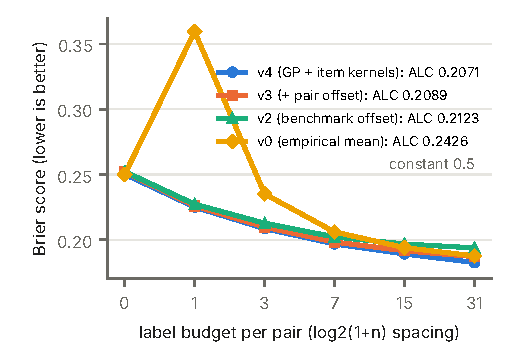
\includegraphics[width=0.49\linewidth]{fig_budget.pdf}\hfill
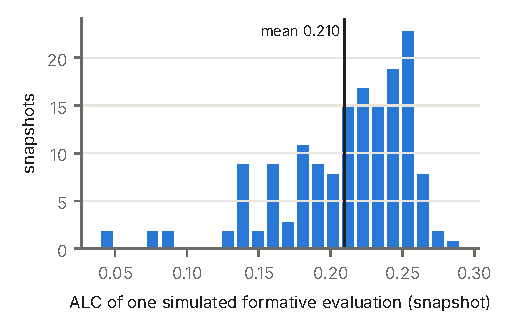
\includegraphics[width=0.49\linewidth]{fig_noise.pdf}
\caption{Left: Brier score per label budget on the local evaluator (Table~\ref{tab:main}). The
unsmoothed empirical mean (v0) is badly hurt at budget 1, where one label gives a prediction of 0 or 1.
Right: distribution of the ALC of one simulated formative evaluation (a snapshot of 3.4 pairs on
average) for v4: mean 0.210, standard deviation 0.047, 5\% quantile 0.135.}
\label{fig:curves}
\end{figure}

\paragraph{Main comparison.} Table~\ref{tab:main} and Figure~\ref{fig:curves} (left) show the
ablation path. Pooling all labels of the benchmark (v2) gives most of the gain over the baselines,
from 0.2426 to 0.2123. A separate pair offset (v3) is worth 0.0034, and the item kernels (v4) a
further 0.0018, mostly at budgets 7 to 31. The GP shrinks low-budget predictions correctly: at budget
1, v4 scores 0.2250 where the unshrunk empirical mean scores 0.3595.

\paragraph{Robustness.} With a per-benchmark split (no item is ever an acquisition item for one
subject and an evaluation item for another), v4 scores 0.2077, v3 0.2093, v0 0.2443 and constant
0.5 scores 0.2500. With a different fold seed (seed 1, per-pair split), v4 scores 0.2085 and v3
0.2105. The ordering of the versions is the same in all three settings.

\paragraph{Sensitivity.} Around the chosen configuration, a calibration multiplier on the
predictive logit (0.9 to 1.3), a scale on the probit variance term (0.6 or 1.0), $\tau_f,\tau_t \in
\{1.0,1.6\}$, $\tau_b \in \{1.0,1.5,2.2\}$, $\tau_p\in\{0.6,1.0,1.4\}$ and an exact-item term
$\tau_e\in\{0,0.7\}$ all give ALC between 0.2071 and 0.2100; none improves on v4. An exact-item term
with $\tau_e=2$ hurts (0.2118 for v3 with it), because it adds prior variance to every prediction
while exact matches across subjects are rare.

\paragraph{Negative result 1: subject ability does not transfer.} For pairs whose model name
appears on other training benchmarks, we correlate the name's mean residual on those benchmarks (pair
logit minus benchmark mean) with its residual on the held-out benchmark: $r=-0.065$ (3,752 pairs, 103
benchmarks). The within-benchmark correlation with release year is only 0.048. The likely reason is
that what a response of 1 means varies: on some benchmarks it is a correct answer, on others a
refusal or a successful attack. The name-based prior therefore makes v1 slightly \emph{worse}
than 0.5 and was removed in v4.

\paragraph{Negative result 2: amortized item difficulty transfers weakly.} A ridge regression on
hashed item features (text unigrams and bigrams, length, media tags, feature tokens), trained on
training benchmarks to predict per-item difficulty logits and evaluated on held-out benchmarks,
reaches a within-benchmark correlation of 0.03 to 0.05 and a benchmark-mean correlation of 0.18 to 0.21.
We did not use it.

\paragraph{How far label pooling can go.} On 2,315 training pairs, knowing each pair's true accuracy
gives Brier 0.183, and also knowing each item's difficulty from all other subjects gives 0.121. Our
$B_{31}$ of 0.1825 is at the first level. Most of the remaining gap is item-level information, which
neither the labels of a few peers nor the item text supplies for a new benchmark.

\paragraph{Prior mean and the hard regime (v5).} Several public entries report that the pairs in
formative draws are harder than the training average. \citet{gpirt} reports a mean accuracy of 0.35
in formative draws and centres the level prior at $-0.6$ logit; \citet{paiksca} and
\citet{doctawho} ship level-prior means of $-1.0$ and $-2.5$. We cannot see the test pool, so
we evaluated a shift $\delta$ of the prior mean under two regimes: our 541 held-out pairs as they
are, and the same pairs reweighted ($w\propto e^{-\lambda a}$ in the pair's evaluation accuracy $a$,
effective sample size 416) to a mean accuracy of 0.35. For $\delta = 0, -0.3, -0.6, -0.8, -1.0, -1.4$,
ALC is 0.2071, 0.2073, 0.2079, 0.2085, 0.2092, 0.2112 unweighted and 0.1922, 0.1906, 0.1893,
0.1887, 0.1882, 0.1878 in the hard regime. Almost all of the gain is at budgets 0 and 1 (hard-regime
$B_0$ 0.2492 for v4 against 0.2301 for v5). We submit $\delta=-0.8$ (v5). It costs 0.0014 if the test
pool resembles the training pool and gains 0.0035 if it is as hard as reported, so it pays off
in expectation whenever the probability of the hard regime exceeds 0.29. The per-benchmark split
gives the same picture (0.2090 against 0.2077 unweighted, 0.1885 against 0.1920 hard).
Weighting training pairs by their response count also gives a mean accuracy of 0.35, but on an
effective sample of only 6 pairs, so we do not rely on it. Building snapshots only from held-out benchmarks
with pool accuracy below 0.45 (``hard world'', 210 pairs) or at least 0.6 (``easy world'', 183
pairs) gives the same picture with v6. The shift is worth about 0.007 in the hard world (0.1813
against 0.1881 without it) and costs about 0.009 in the easy world (0.2074 against 0.1982). We also
tried estimating the pool's difficulty at test time from the other benchmarks' revealed labels
(a hierarchical prior on the shift with standard deviation 0.5 or 1.0). It changed ALC by at most
0.0006 in either world, because a formative-sized draw holds too few other benchmarks, so we did not
use it.

\paragraph{Semantic kernel (v6).} Sentence embeddings help only inside a benchmark. As a
cross-benchmark difficulty prior (ridge from the embedding to an item's difficulty, trained on the
training folds), they predict difficulty on held-out benchmarks no better than hashed text:
within-benchmark correlation 0.02, benchmark-level correlation 0.17. As a kernel between the
revealed items and the target within the benchmark, they lower ALC by 0.00098 relative to v5
(paired over the 541 pairs, standard error 0.00026, benchmark-clustered 0.00042; 54\% of pairs
improve). Under the per-benchmark split the difference is 0.00077 (clustered standard error 0.00030),
and in the hard regime 0.1877 against 0.1887. The gain is concentrated at budgets 7 to 31 ($B_{31}$
0.1798 against 0.1825), where enough labels exist to learn which kinds of item are hard. A
short-range ``near-duplicate'' kernel on raw embedding cosine added nothing (+0.0001).

\paragraph{LLM judge (v7).} On a stratified sample of 1,812 training items (12 per benchmark),
the judge's rating correlates with true item difficulty (mean response over the pool subjects) at
0.195 within benchmarks (mean over 150 benchmarks) and 0.26 at the benchmark level for Haiku 5.5. For
Sonnet 5.5 the figures are 0.242 and 0.33. Embeddings and hashed text reach only 0.02 to 0.04 within
benchmarks. With ratings for 54,341 of the 54,675 item texts used by the evaluator, adding the Haiku
judge to v6 gives ALC 0.2046 / 0.2031 / 0.2036 / 0.2026 / 0.2046 / 0.2053 for
$(s,\tau_j)=(1,0),(1,0.6),(2,0),(2,0.6),(3,0),(3,0.6)$. The chosen setting improves on v6 by 0.00489
(paired standard error 0.00067, benchmark-clustered 0.00121; 59\% of pairs improve), with the largest
gains at low budgets ($B_0$ 0.2495, $B_1$ 0.2224). In the hard regime it scores 0.1840 against v6's
0.1877.
With Sonnet 5.5 ratings (53,664 of 54,675 texts rated; the rest count as unrated), the same model
scores 0.2002 / 0.1998 / 0.2034 for $s=1.5, 2, 3$ ($\tau_j=0.6$). v8 ($s=2$) improves on v6 by 0.00767
(paired standard error 0.00074, benchmark-clustered 0.00146; 67\% of pairs improve) and on the
Haiku judge by 0.00278 (clustered standard error 0.00087). Per budget it scores $B_0$ 0.2453, $B_1$
0.2187, $B_3$ 0.2013, $B_7$ 0.1893, $B_{15}$ 0.1804 and $B_{31}$ 0.1734, and 0.1817 in the hard
regime. With the judge on, the prior shift of $-0.8$ remains the better bet (with Haiku: $-0.4$,
$-0.8$, $-1.2$ give 0.2014, 0.2026, 0.2066 unweighted and 0.1851, 0.1840, 0.1862 in the hard
regime).

\paragraph{In-context judge (v9).} A full cross-validation of the in-context judge would need one
long API call per evaluation item and budget (about 300,000 calls), so we validated it on a subset.
The evaluator dumped, for 46 held-out pairs (26 benchmarks; first 2 snapshots of each fold; 25
evaluation items per pair; budgets 1 to 31), v8's prediction together with the exact revealed context
v8 saw: 5,750 predictions. On these, the budget-weighted Brier (ALC weights over budgets 1 to 31;
budget 0 is unchanged) is 0.2003 for v8, 0.1896 for the in-context Sonnet judge alone and 0.1891 for
their average. The gain is largest at low budgets: at $n=1$, 0.2469 for v8 against 0.2261 for the
judge, because one or two revealed outcomes already tell the LLM what outcome 1 means and how
strong the system is. At $n=31$ the two are equal alone (0.1890, 0.1895) and better averaged
(0.1840). Paired over pairs, the 0.5 average improves on v8 by 0.0109 (standard error 0.0029; 70\%
of pairs). A fixed weight of 0.65 gives 0.0120 (0.0035), with the same value on both halves of the
benchmarks (0.0123 and 0.0116); budget-specific weights chosen on one half and tested on the other
gave 0.0114. Haiku 5.5 as the in-context judge gains 0.0077, and adding it to Sonnet gains 0.0003
more, so v9 uses Sonnet alone. The runtime prompt is byte-identical to the validated one on all
5,750 records. A second, disjoint set of 51 pairs (the next two snapshots of each fold) gives a
smaller gain: v8 scores 0.1460 there (easier pairs), and the average with the judge improves it by
0.0038. Pooled over both sets (97 pairs), the weight-0.65 blend improves on v8 by 0.0077 (standard
error 0.0021; 63\% of pairs improve), and weights from 0.3 to 0.65 all help (0.0053 to 0.0077). We
report 0.0077 as v9's estimated gain. It comes from a subset, not a full cross-validation like the
results for v0 to v8. At budget 0 the same prompt with an empty context still helps, because the LLM
sees the target system's name with the item. On 1,455 budget-0 predictions (97 pairs), v8 scores
0.2533, the judge alone 0.2317, and the 0.65 blend improves $B_0$ by 0.0244 (standard error 0.0064;
consistent across benchmark halves). That is 0.0024 of ALC, used in v10, for an estimated total of
about 0.010 below v8. Finally, Opus 5.5 is a better in-context judge than Sonnet 5.5 at low budgets.
Over budgets 1, 3 and 7 (ALC-weighted), using Opus with weight 0.8 instead of Sonnet with weight
0.65 improves on v10's blend by 0.0040 (standard error 0.0015) on the first probe set and by 0.0038
(0.0014) on the disjoint second set. v11 uses Opus there and Sonnet elsewhere, an estimated 0.014 below
v8 in total. Opus calls are slower (about 3 to 5 s), so v11's per-process time budget for in-context
calls is 45 minutes. At budget 0 Opus adds only 0.0006 of ALC over Sonnet, so we kept Sonnet there.
Computed directly per pair over all budgets, v11 improves on v8 by 0.0140 (standard error 0.0027) on
the 97 probe pairs. The gain shrinks on hard pairs: reweighted to a mean accuracy of 0.35 it is
0.0070 (effective sample size 68), because the LLM judges help most on pairs of intermediate accuracy.
If the hidden test is as hard as reported, v11's real gain over v8 may be nearer 0.007.

\paragraph{A packaging bug found by review.} An independent review of the submission's runtime
found that the official-style loader restores \texttt{sys.path} after importing \texttt{model.py}.
Our lazy imports of the embedding and judge modules inside \texttt{predict} therefore failed
silently on Codabench, so the formative runs of v6 and v7 did not use the semantic kernel or the
judge. We now bind those modules at import time, and our smoke test restores \texttt{sys.path} like
the official checker. The same review led to a negative cache, a circuit breaker and a deadline for
judge calls, so that API failures degrade the model to v6 instead of exceeding time limits.

\paragraph{Leaderboard noise.} One formative evaluation samples at most 1,000 subject-item pairs, so
it scores only a few pairs. On our evaluator, the ALC of a single snapshot of v4 has a standard
deviation of 0.047 (Figure~\ref{fig:curves}, right). The expected best of 10 independent submissions of
the \emph{same} model is 0.124, and of 20 it is 0.098, against a mean of 0.210. Differences between
leaderboard entries of a few hundredths therefore say little about the underlying methods, and
model selection should rely on many pairs. Our submitted model is v10 (Codabench submission \CODABENCHID, formative score \CODABENCHSCORE).
v7 scored 0.1639 on one draw (submission 1039214).
The same v6 archive scored 0.1491 and 0.1651 on two formative draws, a direct illustration of this noise. Earlier versions scored 0.1835 (v4b, submission 1038965) and 0.1543 (v5, submission 1038991) on
one formative draw each. Each draw samples different pairs, so the two numbers are not a paired
comparison of v4b and v5, but both lie within the spread of Figure~\ref{fig:curves} (right).

\section{Limitations}

The local evaluator is our reading of the protocol. The real item sampling per pair, the number of
subjects per benchmark in a formative evaluation and the composition of the test pool may differ,
and absolute scores may shift with them. Hyperparameters were selected on the same cross-validation
used for reporting. The selection effect is small next to the differences we interpret (the
configurations near the optimum differ by less than 0.001, about one third of a standard error), but
it is not zero. Our item-level component helps only a little, and the large gap to the item oracle
remains. We use random acquisition only. A small sentence encoder helps only within a benchmark.
The LLM judge does transfer, but its ratings are noisy (correlation about 0.2), it does not know
each benchmark's labelling convention (for some benchmarks a response of 1 means a refusal or a
successful attack), it makes the predictions depend on an external API (nondeterministic outputs,
latency, and cost: roughly \$0.30 per formative run with Haiku 5.5 and \$5 to \$7 with Sonnet 5.5),
and its prompt was not tuned. The judge sees only the item, not the subject or the revealed labels;
conditioning on either could help but would multiply the number of calls. Subject information is essentially
unused, because what we tried did not transfer.

\section{Reproducibility}

Code: \REPOURL\ (MIT license). The README lists every command. Download the tables with an HF token
(\texttt{tools/download\_data.py}), build the training set and evaluation cache
(\texttt{tools/build\_dataset.py}, \texttt{tools/build\_cache.py}), export the MiniLM weights and embed the evaluation pool
(\texttt{tools/export\_minilm.py}, \texttt{tools/embed\_pool.py}), fit and package a version
(\texttt{tools/make\_submission.py}, \texttt{tools/build\_zip.py}), validate it with the official
checker and our smoke test, and run the local evaluator (\texttt{eval/simulate.py}, about 20\,s on 4
CPUs). All seeds are fixed, and every number in this report comes from files in \texttt{eval/results/}
written by those scripts. The figures are generated by \texttt{report/make\_figures.py}.

\section{Disclosure}

Training data: only \texttt{aims-foundations/measurement-db} \citep{measurementdb}. No external data
is used. At scoring time, v9 (like v8) calls the Anthropic API (Claude Sonnet 5.5; v7 uses Claude Haiku 5.5),
an inference API permitted by the rules, without web search or tools, to rate items. The same API
rated the training items offline for validation (Claude Haiku 5.5 and Claude Sonnet 5.5). The API
key is not part of the released code. One pretrained model is used, frozen, as a text encoder:
\texttt{sentence-transformers/all-MiniLM-L6-v2} \citep{reimers2019,wang2020minilm} (Apache-2.0).
Its weights are converted for our numpy implementation and bundled with the submission. The archive validator and
streaming client helper are copied unchanged from the official baseline repository
\citep{paiec_baselines} (MIT). The empirical-mean baseline (v0) is that repository's predictor. We
did not use code from other teams. The idea of lowering the level prior for the hard
test regime comes from public entries \citep{gpirt,paiksca,doctawho}, found through an LLM-assisted
literature and repository search, and was validated on our own evaluator before use. An LLM coding assistant (Claude Code, Anthropic) was used
throughout development (data pipeline, evaluator, model code, experiments) and to draft this report.
The author reviewed the outputs, and every reported number was produced by the released scripts.

\begin{thebibliography}{14}

\bibitem[Brier(1950)]{brier1950}
G.~W. Brier.
\newblock Verification of forecasts expressed in terms of probability.
\newblock \emph{Monthly Weather Review}, 78(1):1--3, 1950.

\bibitem[MacKay(1992)]{mackay1992}
D.~J.~C. MacKay.
\newblock The evidence framework applied to classification networks.
\newblock \emph{Neural Computation}, 4(5):720--736, 1992.

\bibitem[{AIMS}(2026{\natexlab{a}})]{measurementdb}
AIMS Foundations.
\newblock The {AI} Measurement Data Bank (measurement-db).
\newblock Hugging Face dataset \texttt{aims-foundations/measurement-db}, 2026.

\bibitem[{AIMS}(2026{\natexlab{b}})]{paiec_site}
Stanford AI Measurement Science.
\newblock The Predictive {AI} Evaluation Competition at {NeurIPS} 2026.
\newblock \url{https://aims.stanford.edu/competition}, 2026.

\bibitem[doctawho42(2026)]{doctawho}
doctawho42.
\newblock {PAIEC} entry (hierarchical {IRT} with a level prior).
\newblock \url{https://github.com/doctawho42/PAIEC}, 2026.

\bibitem[nguefackuriel(2026)]{gpirt}
nguefackuriel.
\newblock paiec-gpirt: {GP-IRT} fitted at test time.
\newblock \url{https://github.com/nguefackuriel/paiec-gpirt}, 2026.

\bibitem[paiksca(2026)]{paiksca}
paiksca.
\newblock {PAIEC} 2026: a benchmark level prior learned from 182 public benchmarks.
\newblock \url{https://github.com/paiksca/paiec-2026}, 2026.

\bibitem[Rasmussen and Williams(2006)]{rasmussen2006}
C.~E. Rasmussen and C.~K.~I. Williams.
\newblock \emph{Gaussian Processes for Machine Learning}.
\newblock MIT Press, 2006.

\bibitem[Reimers and Gurevych(2019)]{reimers2019}
N.~Reimers and I.~Gurevych.
\newblock Sentence-{BERT}: sentence embeddings using {S}iamese {BERT}-networks.
\newblock In \emph{Proceedings of EMNLP-IJCNLP}, 2019.

\bibitem[Robbins(1956)]{robbins1956}
H.~Robbins.
\newblock An empirical {B}ayes approach to statistics.
\newblock In \emph{Proceedings of the Third Berkeley Symposium on Mathematical Statistics and Probability}, 1956.

\bibitem[Truong et~al.(2026)]{paiec_baselines}
S.~Truong, W.~Salaudeen, N.~Truong, S.~Wang, A.~Wang, L.~Guerdan, Z.~Xiao, X.~Xie, N.~Haber, and S.~Koyejo.
\newblock {PAIEC} predictor baselines.
\newblock \url{https://github.com/aims-foundations/paiec_baseline}, 2026.

\bibitem[Wang et~al.(2020)]{wang2020minilm}
W.~Wang, F.~Wei, L.~Dong, H.~Bao, N.~Yang, and M.~Zhou.
\newblock {MiniLM}: deep self-attention distillation for task-agnostic compression of pre-trained transformers.
\newblock In \emph{Advances in Neural Information Processing Systems}, 2020.

\bibitem[Williams and Barber(1998)]{williams1998}
C.~K.~I. Williams and D.~Barber.
\newblock {B}ayesian classification with {G}aussian processes.
\newblock \emph{IEEE Transactions on Pattern Analysis and Machine Intelligence}, 20(12):1342--1351, 1998.

\end{thebibliography}

\end{document}
